\chapter{Approach}
\label{ch:approach}

% \instructions{Page budget for Approach: 20-30 pages
% %
% \begin{itemize}
%     \item This chapter describes your main contributions (i.e., what you did) and the decisions that went into them (i.e., why did you did it the way you did it).
%     \item Alternative headings may be used depending on the kind of contribution(s) you make.
% \end{itemize}
% }

\section{Overview}
% \instructions{
% \begin{itemize}
%     \item This section should explain the high-level design
%     \item Include possibly an architecture figure that shows how the different parts fit together and what processing/technology/tools/datasets have been used for the different components.
% \end{itemize}
% %
% Name these themes based on the different components or sub-problems you are solving in your thesis.
% }

The TEX2BEAM system can generate LaTeX Beamer format presentations from academic research papers. It consists of three primary components: a report parser, a presentation generator, and a presentation compiler. The report parser extracts the essential information from the report, the presentation generator creates the presentation, and the presentation compiler assembles the presentation into a LaTeX Beamer file. The system is designed to be modular, allowing each component to be replaced with a different implementation. This feature enables easy expansion of the system, as well as convenient testing of various approaches.

To generate slides, a suggested two-step approach is: first, identify high-level topics and generate slide titles, and second, generate bullet points for each slide. A third step can be taken to create visual content like tables and illustrations for the slides if needed.

\begin{figure}
    \centering
    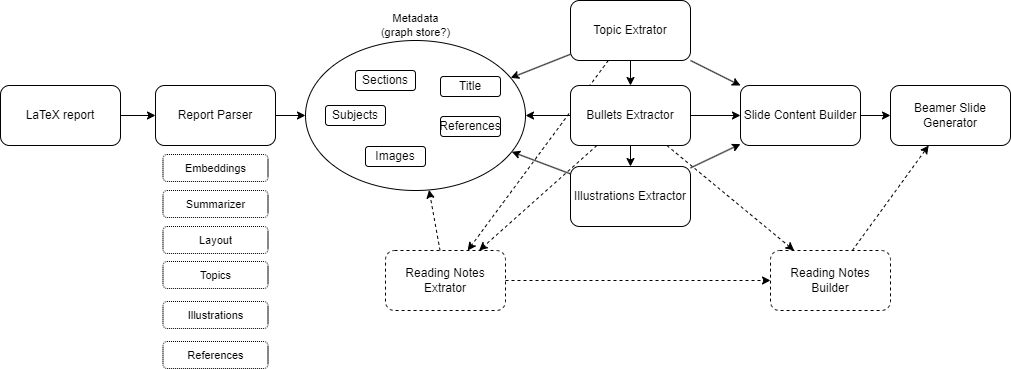
\includegraphics[width=1\linewidth]{images/High-Level Architecture Diagram.png}
    \caption{High-level architecture.}
    \label{fig:high-level-architecture}
\end{figure}

%
\subsection{NOTES (Section to be deleted)}
\begin{itemize}
    \item Could it be beneficial to use a knowledge graph to represent the information in the report? This could be used to generate the presentation and provide a visual representation of the information in the report.
    \item Summarizing vs extracting information from the report. How do we decide the best approach?
    \item Should we test various models, e.g., HuggingFace transformers vs ChatGPT?
    \item Testing how well already existing models (e.g., ChatGPT, MS Copilot) perform when asked to generate a presentation from a research paper.
    \item How do we identify the main file when using LaTeX as the source file? Where do we start parsing? 
    \item Extract the outline from PDF/PPT titles, add additional metadata (e.g., bullets, tables, illustrations), and generate slides from an outline. (Few-shot prompting LLM?) (Manually procure a high-quality dataset)
\end{itemize}

\section{Dataset}
This thesis aims to automate the creation of LaTeX Beamer presentations from LaTeX research papers.

One of the key contributions of this thesis is the development of a dataset that will be used to train and evaluate the system. The dataset will be created by collecting research papers and their corresponding presentations from various sources. While it is ideal to have both the reports and presentations in LaTeX format, finding them in the required format in practice has been challenging. As a result, the dataset will contain reports in LaTeX format and presentations in PDF format.

Although some datasets are available, they are not formatted as we need. However, they can create the dataset by utilizing the presentations and extracting the corresponding research papers in the required format. To obtain research papers in the required format, we can mine the arXiv archive since it is a trustworthy source for such papers. If we plan to publish the dataset, adhering to copyright laws for the scraped data is crucial. Additionally, we must follow the data scraping guidelines provided by arXiv.

\subsection{Data Collection Methodology}
We must find sources that fulfill the prerequisite to create a dataset of research papers and presentations in LaTeX format. The arXiv archive is a suitable source for research papers in LaTeX format. However, obtaining corresponding presentations in LaTeX Beamer format has been challenging. Most authors do not publish presentations for their research papers. After visiting the personal websites of several authors, we found that the ratio of presentations to research papers was less than 1:10. Therefore, we decided to start with the presentations and mine corresponding research papers in the required format. Additionally, the few available presentations are often in PDF or PPT format, which must be converted to the required format. 

Our data collection process is based on the conference papers from the dataset provided by Fu:2022:AAAI. We created a web scraper using the Python Scrapy framework to automate this process. The scraper starts by searching for links to presentations in the event archives. We use the Python arXiv library for each presentation found to search for the corresponding research paper in the arXiv archive. If we find an exact match between the titles from both sources, we download the presentation in PDF format and the matched paper in PDF and source format. However, we need to check the source files because they may not be guaranteed to be in LaTeX format before using them in later processing.

We will manually add some papers and presentations to the dataset to ensure that the dataset is high quality and representative of the research papers and presentations on which the system will be used. This will also help ensure the dataset is diverse enough to meet the system's requirements.

\subsection{Extracting data from PDF documents}
We need to convert the PDF presentations into a suitable format to create a training dataset that can be used to train and optimize a model for generating LaTeX Beamer presentations. However, extracting valid, structured data from PDF documents can be difficult because they are designed in a fixed-layout format. This means that the text is not stored in a structured way, making it challenging to extract both the text and the document's structure. 

We have not identified any tool that can produce the required output to generate the dataset.  Text and images can be extracted using tools like pdfminer.six or PyMuPDF, but we need to add metadata to identify the type of text, like headings, bullets, body text, etc. Other tools aim to convert the PDF into formats like PPT and DOCX by preserving content and layout, but this is still only for visual representation, not adding our required metdata.

While tools are available to extract text and objects from PDF documents, much of the PDF document's layout and formatting information is unavailable. Therefore, it must be inferred from the context of expected formatting. 

Some examples of expected formatting are:

\begin{itemize}
    \item \textbf{Title}: The title of a presentation is usually placed at the top of the slide and is visually distinct from the rest of the text. When we extract text from a PDF document, we can determine if the first line of text is the slide's title by its position. However, this method may not work for slides with multi-line titles or no titles.
    \item \textbf{Bullet points}: Bullet points are easily identifiable visually, but text extraction tools may not recognize them. The reason is that authors are free to use any bullet point style they prefer, whether in the form of a list or a series of lines with a bullet point character at the start. This makes it challenging to extract bullet points in a structured way. 
    \item \textbf{Tables}: The text is organized in a cell or grid structure, with optional headings and row names. Pure text extraction will leave out essential formatting details and may even break the content order. 
    \item \textbf{Image and table captions}: This text should be linked to their respective image or table and not considered stand-alone.
\end{itemize}

Several methods for converting the PDF presentations into a usable dataset have been considered:

\begin{itemize}
    \item \textbf{Manually recreate the presentations in Beamer format}: Although this option could create high-quality output, it will also be time-consuming. We don't consider this a practical alternative since we want to have as large a dataset as possible.
    \item \textbf{Existing tools, like pdf2latex or pdf2docx}: These tools can extract much of the content, but since they cannot extract required metadata, additional work will be required.
    \item \textbf{Bespoke machine learning model, created and trained from scratch}: This has been demonstrated in previous works and would be a potential way forward. However, this would require a large amount of training data, substantial computing resources, and time to train the model. This would have likely been the best potential method a few years ago. However, with the availability of pre-trained and large language models (LLM's), these other options will likely be better than we can produce on out own.
    \item \textbf{Fine-tune transformer model, e.g., BERT or T5 from Huggingface}: Pre-trained transformer models for various NLP tasks are publicly available for download, use, and fine-tuning from websites like Huggingface. These models are often trained on large datasets utilizing extensive computing resources and time. Depending on the model, they may do an excellent job out of the box, while improvements can be made by fine-tuning the model on our dataset.
    \item \textbf{LLM, e.g .chatGPT, possibly fine-tune if required}: Some of the most significant LLM's today are provided by big-tech coprorations, like Microsoft, Google, and OpenAI.
\end{itemize}

The proposed method combines multiple steps to produce the required \LaTeX{} Beamer presentations:
\begin{itemize}
    \item \textbf{Step 1}: Use pdf2docx\footnote{\url{https://github.com/ArtifexSoftware/pdf2docx}} to read and parse the PDF presentation contents. This package use the PyMuPDF package in the background and have added some additional parsing logic that helps identify e.g. blocks of text, and images. The output from this step is a JSON object that contains all the layout and content information extracted from the PDF file.
    \item \textbf{Step 2}: Extract the text content from the output from step 1. The output from this step is JSONL that contains a list of strings for each slide.
    \item \textbf{Step 3}: Use ChatGPT to analyze and parse the output from step 2 to (re-)create the \LaTeX{} Beamer presentation that would resemble the original PDF file content as closely as possible.
\end{itemize}

\subsection{Data Augmentation}
Enriching the dataset with details such as internal and external references, tables, and illustrations may be helpful. This can help generate the presentation, as it can be used to determine which additional items to include together with the text.


\section{Tools}

\subsection{\LaTeX{}}
Parsing \LaTeX{} documents may be done using the TexSoup Python library\footnote{\url{https://texsoup.alvinwan.com/}}.

\subsection{PDF}
Several tools may be able to convert PDF files into text or \LaTeX{} format: 

\begin{itemize}
    \item \textbf{pdf2docx}\footnote{\url{https://pdf2docx.readthedocs.io/}} - ''pdf2docx is a Python library to extract data from PDF with PyMuPDF, parse layout with rule, and generate docx files with python-docx.''
    \item \textbf{PyMuPDF}\footnote{\url{https://pymupdf.readthedocs.io/}} - ''PyMuPDF is a high performance Python library for data extraction, analysis, conversion \& manipulation of PDF (and other) documents.''
    \item \textbf{Pdfminer.six}\footnote{\url{https://github.com/pdfminer/pdfminer.six}} - ''Pdfminer.six is a community maintained fork of the original PDFMiner. It is a tool for extracting information from PDF documents. It focuses on getting and analyzing text data.''
    \item \textbf{GROBID}\footnote{\url{https://github.com/kermitt2/grobid}} - ''A machine learning software for extracting information from scholarly documents''
    \item \textbf{PDFMiner}\footnote{\url{https://pypi.org/project/pdfminer/}} - (no longer maintained; see Pdfminer.six) PDFMiner is a tool for extracting information from PDF documents. Unlike other PDF-related tools, it focuses entirely on getting and analyzing text data. PDFMiner lets one obtain the exact text location on a page and other information, such as fonts or lines. It includes a PDF converter that can transform PDF files into other text formats (such as HTML). It has an extensible PDF parser that can be used for purposes other than text analysis.
    \item \textbf{pdftolatex}\footnote{\url{https://github.com/vinaykanigicherla/pdftolatex}} - ''Python tool for generating \LaTeX{} code from PDF files.''
    \item \textbf{pdf2latex-converter}\footnote{\url{https://github.com/mcpeixoto/pdf2latex-converter}} - ''Originally based on \textbf{pdftolatex}.'' (Work in progress).
    \item \textbf{pdf2latex}\footnote{\url{https://github.com/emsquid/pdf2latex}} - ''pdf2latex is a CLI tool to convert a PDF back to LaTeX.''
    \item \textbf{pdf2latex}\footnote{\url{https://github.com/safnuk/pdf2latex}} - ''Train a neural network to produce latex source code which generates a given pdf file.''
    \item \textbf{PDF2LaTeX}\footnote{\url{https://github.com/senyalin/PDF2LaTeX}} - PDF2LaTeX is a tool for converting PDF files into \LaTeX{} format. It is a command-line tool that can convert PDF files into \LaTeX{} format. It is written in Python and uses the PyPDF2 library to parse PDF files. It can be used to convert PDF files into \LaTeX{} format.
    \item \textbf{pypdf}\footnote{\url{https://pypi.org/project/pypdf/}} - pypdf is a Python library for working with PDF files. It can extract text from PDF files and convert PDF files into other formats (such as HTML).
    \item \textbf{pdfly}\footnote{\url{https://github.com/py-pdf/pdfly}} - ''CLI tool to extract (meta)data from PDF and manipulate PDF files.''
    \item PyMuPDF
\end{itemize}

\section{Baseline}
We use the dataset and trained models provided by \citet{Fu:2022:AAAI} to set a baseline for the system. The dataset contains 5873 pairs of research papers and presentations, and the authors have published their trained models and the complete dataset online. As shown in Table \ref{table:dataset}, the reports are in PDF format, and the presentation slides are in JPEG format. 

\section{Method}
The outline of the method is as follows:

\begin{enumerate}
\item Parse the \LaTeX{} report and extract the relevant information.
    \begin{itemize}
        \item Use tools like TexSoup or pylatex to parse the \LaTeX{} document.
        \item Extract metadata such as title, authors, and abstract.
        \item Extract the main sections and subsections of the report.
        \item Extract the text from the report.
        \item Extract the tables and illustrations from the report.
    \end{itemize}
    (Consider if this should be a "simple" structure/class or if using a knowledge graph to represent the information in the report could be helpful.)

\item Identify the main topics/sections in the report.
    \begin{itemize}
        \item Use the extracted sections and subsections to identify the main topics.
        \item If using a knowledge graph, consider if it could be used to identify the main topics.
    \end{itemize}

\item Summarize each section and generate bullet points.
    \begin{itemize}
        \item Use a summarizing model to summarize the text from each section.
        \item Generate bullet points from the summarized text.
    \end{itemize}

\item (optional) Generate speaking notes

\item Identify relevant visual content, such as tables and illustrations.
    \begin{itemize}
        \item Use a model to identify the relevant visual content for the slides.
    \end{itemize}
    
\item (optional) Generate visual content for the slides.
    \begin{itemize}
        \item Use a model to generate visual content for the slides.
    \end{itemize}

\item Split the bullet points and visual content into slides.
    \begin{itemize}
        \item Use the bullet points and visual content to generate the slides.
    \end{itemize}

\item Generate the presentation in \LaTeX{} Beamer format.
    \begin{itemize}
        \item Select appropriate templates for the slides.
        \item Use a template to generate the presentation in \LaTeX{} Beamer format.
        \item Compile the presentation into a PDF file (?)
    \end{itemize}
\end{enumerate}

\section{Limitations}
To limit the scope of this project and to make it feasible to complete within the given time frame, we have made the following limitations:
\begin{itemize}
    \item 
\end{itemize}

\subsection{Report Parser (RP)}
The \emph{Report Parser (RP)} is responsible for extracting the relevant information from the report. The report parser comprises two main components: the \emph{Report Content Extractor (RCE)} and the \emph{Report Content Summarizer (RCS)}. The \emph{Report Content Extractor} is responsible for extracting the relevant information from the report, while the \emph{Report Content Summarizer} summarizes the extracted data.

\subsection{Presentation Content Generator}
The \emph{Presentation Content Generator (PCG)} is responsible for 
Presentations can be generated in various layouts, content, and style variations. 

\subsection{Presentation Slides Generator}
There are several options for generating visual layout and content for the presentation slides. 

To keep things simple, we propose three simple slide layouts: A title slide, a bullet point slide, and a visual slide. The title slide will contain the title, the bullet point slide will contain a list of bullet points, and the visual slide will represent the information in the report.

\section{Evaluation}
The system will be evaluated on how well it can extract the relevant information from the report and how well it can summarize it in a presentation. The evaluation will be done by comparing the generated presentations with the original presentations. The evaluation will use metrics such as BLEU, ROUGE, and METEOR. The system will also be evaluated on how well it can identify the visual content for the slides, such as tables and illustrations.

% \instructions{
% \begin{itemize}
%     \item For larger/more complex projects, the separate themes may be chapters on their own (e.g., components in a system; sub-problems of a major evaluation study; etc.).
%     \item Include screenshots, examples, tables, algorithms (with pseudo code), plots for some preliminary observations leading to some aspect of your approach decisions, etc. so that it's not just text.
%     \item Always discuss the alternatives considered and the rationale for the choosing the solutions you adopted.
% \end{itemize}
% }
% %
